%\title{ICINCO '14: Adaptive Extended Kalman Filter for Vehicle Attitude Estimation with Low Cost Sensors}
%% bare_jrnl.tex
%% V1.4
%% 2012/12/27
%% by Michael Shell
%% see http://www.michaelshell.org/
%% for current contact information.
%%
%% This is a skeleton file demonstrating the use of IEEEtran.cls
%% (requires IEEEtran.cls version 1.8 or later) with an IEEE journal paper.
%%
%% Support sites:
%% http://www.michaelshell.org/tex/ieeetran/
%% http://www.ctan.org/tex-archive/macros/latex/contrib/IEEEtran/
%% and
%% http://www.ieee.org/



% *** Authors should verify (and, if needed, correct) their LaTeX system  ***
% *** with the testflow diagnostic prior to trusting their LaTeX platform ***
% *** with production work. IEEE's font choices can trigger bugs that do  ***
% *** not appear when using other class files.                            ***
% The testflow support page is at:
% http://www.michaelshell.org/tex/testflow/


%%*************************************************************************
%% Legal Notice:
%% This code is offered as-is without any warranty either expressed or
%% implied; without even the implied warranty of MERCHANTABILITY or
%% FITNESS FOR A PARTICULAR PURPOSE! 
%% User assumes all risk.
%% In no event shall IEEE or any contributor to this code be liable for
%% any damages or losses, including, but not limited to, incidental,
%% consequential, or any other damages, resulting from the use or misuse
%% of any information contained here.
%%
%% All comments are the opinions of their respective authors and are not
%% necessarily endorsed by the IEEE.
%%
%% This work is distributed under the LaTeX Project Public License (LPPL)
%% ( http://www.latex-project.org/ ) version 1.3, and may be freely used,
%% distributed and modified. A copy of the LPPL, version 1.3, is included
%% in the base LaTeX documentation of all distributions of LaTeX released
%% 2003/12/01 or later.
%% Retain all contribution notices and credits.
%% ** Modified files should be clearly indicated as such, including  **
%% ** renaming them and changing author support contact information. **
%%
%% File list of work: IEEEtran.cls, IEEEtran_HOWTO.pdf, bare_adv.tex,
%%                    bare_conf.tex, bare_jrnl.tex, bare_jrnl_compsoc.tex,
%%                    bare_jrnl_transmag.tex
%%*************************************************************************

% Note that the a4paper option is mainly intended so that authors in
% countries using A4 can easily print to A4 and see how their papers will
% look in print - the typesetting of the document will not typically be
% affected with changes in paper size (but the bottom and side margins will).
% Use the testflow package mentioned above to verify correct handling of
% both paper sizes by the user's LaTeX system.
%
% Also note that the "draftcls" or "draftclsnofoot", not "draft", option
% should be used if it is desired that the figures are to be displayed in
% draft mode.
%
\documentclass[conference]{IEEEtran}
%
% If IEEEtran.cls has not been installed into the LaTeX system files,
% manually specify the path to it like:
% \documentclass[journal]{../sty/IEEEtran}

% Some very useful LaTeX packages include:
% (uncomment the ones you want to load)


% *** MISC UTILITY PACKAGES ***
%
%\usepackage{ifpdf}
% Heiko Oberdiek's ifpdf.sty is very useful if you need conditional
% compilation based on whether the output is pdf or dvi.
% usage:
% \ifpdf
%   % pdf code
% \else
%   % dvi code
% \fi
% The latest version of ifpdf.sty can be obtained from:
% http://www.ctan.org/tex-archive/macros/latex/contrib/oberdiek/
% Also, note that IEEEtran.cls V1.7 and later provides a builtin
% \ifCLASSINFOpdf conditional that works the same way.
% When switching from latex to pdflatex and vice-versa, the compiler may
% have to be run twice to clear warning/error messages.

\usepackage[pdftex,
            pdfauthor={tbd, tbd, tbd},
            pdftitle={EPE and Speed Adaptive Extended Kalman Filter for Vehicle Position and Attitude Estimation with Low Cost GNSS and IMU Sensors},
            pdfsubject={EPE and Speed Adaptive Extended Kalman Filter for Vehicle Position and Attitude Estimation with Low Cost GNSS and IMU Sensors},
            pdfkeywords={Kalman, Adaptive, Extended, Filter},
            pdfproducer={Latex with hyperref},
            pdfcreator={writeLaTeX},
            colorlinks=true,
            linkcolor=black,
            citecolor=black,
            filecolor=black,
            urlcolor=black,
            bookmarks=true,
            bookmarksopen=false,
            bookmarksopenlevel=3,
            plainpages=false,
            pdfpagelabels=true]{hyperref}




% *** CITATION PACKAGES ***
%
\usepackage{cite}
% cite.sty was written by Donald Arseneau
% V1.6 and later of IEEEtran pre-defines the format of the cite.sty package
% \cite{} output to follow that of IEEE. Loading the cite package will
% result in citation numbers being automatically sorted and properly
% "compressed/ranged". e.g., [1], [9], [2], [7], [5], [6] without using
% cite.sty will become [1], [2], [5]--[7], [9] using cite.sty. cite.sty's
% \cite will automatically add leading space, if needed. Use cite.sty's
% noadjust option (cite.sty V3.8 and later) if you want to turn this off
% such as if a citation ever needs to be enclosed in parenthesis.
% cite.sty is already installed on most LaTeX systems. Be sure and use
% version 4.0 (2003-05-27) and later if using hyperref.sty. cite.sty does
% not currently provide for hyperlinked citations.
% The latest version can be obtained at:
% http://www.ctan.org/tex-archive/macros/latex/contrib/cite/
% The documentation is contained in the cite.sty file itself.






% *** GRAPHICS RELATED PACKAGES ***
%
\ifCLASSINFOpdf
   \usepackage[pdftex]{graphicx}
  % declare the path(s) where your graphic files are
   \graphicspath{{../images/}{../pdf/}{../jpeg/}}
  % and their extensions so you won't have to specify these with
  % every instance of \includegraphics
   \DeclareGraphicsExtensions{.pdf,.jpeg,.png}
\else
  % or other class option (dvipsone, dvipdf, if not using dvips). graphicx
  % will default to the driver specified in the system graphics.cfg if no
  % driver is specified.
   \usepackage[dvips]{graphicx}
  % declare the path(s) where your graphic files are
   \graphicspath{{../images/}{../eps/}}
  % and their extensions so you won't have to specify these with
  % every instance of \includegraphics
   \DeclareGraphicsExtensions{.eps}
\fi
% graphicx was written by David Carlisle and Sebastian Rahtz. It is
% required if you want graphics, photos, etc. graphicx.sty is already
% installed on most LaTeX systems. The latest version and documentation
% can be obtained at: 
% http://www.ctan.org/tex-archive/macros/latex/required/graphics/
% Another good source of documentation is "Using Imported Graphics in
% LaTeX2e" by Keith Reckdahl which can be found at:
% http://www.ctan.org/tex-archive/info/epslatex/
%
% latex, and pdflatex in dvi mode, support graphics in encapsulated
% postscript (.eps) format. pdflatex in pdf mode supports graphics
% in .pdf, .jpeg, .png and .mps (metapost) formats. Users should ensure
% that all non-photo figures use a vector format (.eps, .pdf, .mps) and
% not a bitmapped formats (.jpeg, .png). IEEE frowns on bitmapped formats
% which can result in "jaggedy"/blurry rendering of lines and letters as
% well as large increases in file sizes.
%
% You can find documentation about the pdfTeX application at:
% http://www.tug.org/applications/pdftex





% *** MATH PACKAGES ***
%
\usepackage[cmex10]{amsmath}
% A popular package from the American Mathematical Society that provides
% many useful and powerful commands for dealing with mathematics. If using
% it, be sure to load this package with the cmex10 option to ensure that
% only type 1 fonts will utilized at all point sizes. Without this option,
% it is possible that some math symbols, particularly those within
% footnotes, will be rendered in bitmap form which will result in a
% document that can not be IEEE Xplore compliant!
%
% Also, note that the amsmath package sets \interdisplaylinepenalty to 10000
% thus preventing page breaks from occurring within multiline equations. Use:
\interdisplaylinepenalty=2500
% after loading amsmath to restore such page breaks as IEEEtran.cls normally
% does. amsmath.sty is already installed on most LaTeX systems. The latest
% version and documentation can be obtained at:
% http://www.ctan.org/tex-archive/macros/latex/required/amslatex/math/





% *** SPECIALIZED LIST PACKAGES ***
%
%\usepackage{algorithmic}
% algorithmic.sty was written by Peter Williams and Rogerio Brito.
% This package provides an algorithmic environment fo describing algorithms.
% You can use the algorithmic environment in-text or within a figure
% environment to provide for a floating algorithm. Do NOT use the algorithm
% floating environment provided by algorithm.sty (by the same authors) or
% algorithm2e.sty (by Christophe Fiorio) as IEEE does not use dedicated
% algorithm float types and packages that provide these will not provide
% correct IEEE style captions. The latest version and documentation of
% algorithmic.sty can be obtained at:
% http://www.ctan.org/tex-archive/macros/latex/contrib/algorithms/
% There is also a support site at:
% http://algorithms.berlios.de/index.html
% Also of interest may be the (relatively newer and more customizable)
% algorithmicx.sty package by Szasz Janos:
% http://www.ctan.org/tex-archive/macros/latex/contrib/algorithmicx/




% *** ALIGNMENT PACKAGES ***
%
\usepackage{array}
% Frank Mittelbach's and David Carlisle's array.sty patches and improves
% the standard LaTeX2e array and tabular environments to provide better
% appearance and additional user controls. As the default LaTeX2e table
% generation code is lacking to the point of almost being broken with
% respect to the quality of the end results, all users are strongly
% advised to use an enhanced (at the very least that provided by array.sty)
% set of table tools. array.sty is already installed on most systems. The
% latest version and documentation can be obtained at:
% http://www.ctan.org/tex-archive/macros/latex/required/tools/


% IEEEtran contains the IEEEeqnarray family of commands that can be used to
% generate multiline equations as well as matrices, tables, etc., of high
% quality.

\usepackage{siunitx}
\sisetup{
  locale = DE ,
  per-mode = symbol
}


% *** SUBFIGURE PACKAGES ***
%\ifCLASSOPTIONcompsoc
%  \usepackage[caption=false,font=normalsize,labelfont=sf,textfont=sf]{subfig}
%\else
%  \usepackage[caption=false,font=footnotesize]{subfig}
%\fi
% subfig.sty, written by Steven Douglas Cochran, is the modern replacement
% for subfigure.sty, the latter of which is no longer maintained and is
% incompatible with some LaTeX packages including fixltx2e. However,
% subfig.sty requires and automatically loads Axel Sommerfeldt's caption.sty
% which will override IEEEtran.cls' handling of captions and this will result
% in non-IEEE style figure/table captions. To prevent this problem, be sure
% and invoke subfig.sty's "caption=false" package option (available since
% subfig.sty version 1.3, 2005/06/28) as this is will preserve IEEEtran.cls
% handling of captions.
% Note that the Computer Society format requires a larger sans serif font
% than the serif footnote size font used in traditional IEEE formatting
% and thus the need to invoke different subfig.sty package options depending
% on whether compsoc mode has been enabled.
%
% The latest version and documentation of subfig.sty can be obtained at:
% http://www.ctan.org/tex-archive/macros/latex/contrib/subfig/




% *** FLOAT PACKAGES ***
%
%\usepackage{fixltx2e}
% fixltx2e, the successor to the earlier fix2col.sty, was written by
% Frank Mittelbach and David Carlisle. This package corrects a few problems
% in the LaTeX2e kernel, the most notable of which is that in current
% LaTeX2e releases, the ordering of single and double column floats is not
% guaranteed to be preserved. Thus, an unpatched LaTeX2e can allow a
% single column figure to be placed prior to an earlier double column
% figure. The latest version and documentation can be found at:
% http://www.ctan.org/tex-archive/macros/latex/base/


%\usepackage{stfloats}
% stfloats.sty was written by Sigitas Tolusis. This package gives LaTeX2e
% the ability to do double column floats at the bottom of the page as well
% as the top. (e.g., "\begin{figure*}[!b]" is not normally possible in
% LaTeX2e). It also provides a command:
%\fnbelowfloat
% to enable the placement of footnotes below bottom floats (the standard
% LaTeX2e kernel puts them above bottom floats). This is an invasive package
% which rewrites many portions of the LaTeX2e float routines. It may not work
% with other packages that modify the LaTeX2e float routines. The latest
% version and documentation can be obtained at:
% http://www.ctan.org/tex-archive/macros/latex/contrib/sttools/
% Do not use the stfloats baselinefloat ability as IEEE does not allow
% \baselineskip to stretch. Authors submitting work to the IEEE should note
% that IEEE rarely uses double column equations and that authors should try
% to avoid such use. Do not be tempted to use the cuted.sty or midfloat.sty
% packages (also by Sigitas Tolusis) as IEEE does not format its papers in
% such ways.
% Do not attempt to use stfloats with fixltx2e as they are incompatible.
% Instead, use Morten Hogholm'a dblfloatfix which combines the features
% of both fixltx2e and stfloats:
%
% \usepackage{dblfloatfix}
% The latest version can be found at:
% http://www.ctan.org/tex-archive/macros/latex/contrib/dblfloatfix/


%\ifCLASSOPTIONcaptionsoff
%  \usepackage[nomarkers]{endfloat}
% \let\MYoriglatexcaption\caption
% \renewcommand{\caption}[2][\relax]{\MYoriglatexcaption[#2]{#2}}
%\fi
% endfloat.sty was written by James Darrell McCauley, Jeff Goldberg and 
% Axel Sommerfeldt. This package may be useful when used in conjunction with 
% IEEEtran.cls'  captionsoff option. Some IEEE journals/societies require that
% submissions have lists of figures/tables at the end of the paper and that
% figures/tables without any captions are placed on a page by themselves at
% the end of the document. If needed, the draftcls IEEEtran class option or
% \CLASSINPUTbaselinestretch interface can be used to increase the line
% spacing as well. Be sure and use the nomarkers option of endfloat to
% prevent endfloat from "marking" where the figures would have been placed
% in the text. The two hack lines of code above are a slight modification of
% that suggested by in the endfloat docs (section 8.4.1) to ensure that
% the full captions always appear in the list of figures/tables - even if
% the user used the short optional argument of \caption[]{}.
% IEEE papers do not typically make use of \caption[]'s optional argument,
% so this should not be an issue. A similar trick can be used to disable
% captions of packages such as subfig.sty that lack options to turn off
% the subcaptions:
% For subfig.sty:
% \let\MYorigsubfloat\subfloat
% \renewcommand{\subfloat}[2][\relax]{\MYorigsubfloat[]{#2}}
% However, the above trick will not work if both optional arguments of
% the \subfloat command are used. Furthermore, there needs to be a
% description of each subfigure *somewhere* and endfloat does not add
% subfigure captions to its list of figures. Thus, the best approach is to
% avoid the use of subfigure captions (many IEEE journals avoid them anyway)
% and instead reference/explain all the subfigures within the main caption.
% The latest version of endfloat.sty and its documentation can obtained at:
% http://www.ctan.org/tex-archive/macros/latex/contrib/endfloat/
%
% The IEEEtran \ifCLASSOPTIONcaptionsoff conditional can also be used
% later in the document, say, to conditionally put the References on a 
% page by themselves.




% *** PDF, URL AND HYPERLINK PACKAGES ***
%
\usepackage{url}
% url.sty was written by Donald Arseneau. It provides better support for
% handling and breaking URLs. url.sty is already installed on most LaTeX
% systems. The latest version and documentation can be obtained at:
% http://www.ctan.org/tex-archive/macros/latex/contrib/url/
% Basically, \url{my_url_here}.



% *** Do not adjust lengths that control margins, column widths, etc. ***
% *** Do not use packages that alter fonts (such as pslatex).         ***
% There should be no need to do such things with IEEEtran.cls V1.6 and later.
% (Unless specifically asked to do so by the journal or conference you plan
% to submit to, of course. )


% correct bad hyphenation here
\hyphenation{op-tical net-works semi-conduc-tor}



%\author{
%\IEEEauthorblockN{Paul Balzer}
%\IEEEauthorblockA{University of Applied Sciences\\
%Dresden, Germany\\
%balzer@htw-dresden.de}
%\and
%\IEEEauthorblockN{Toralf Trautmann}
%\IEEEauthorblockA{University of Applied Sciences\\
%Dresden, Germany\\
%trautmann@mw.htw-dresden.de}
%\and
%\IEEEauthorblockN{Oliver Michler}
%\IEEEauthorblockA{Technical University\\
%Dresden, Germany\\
%oliver.michler@tu-dresden.de}
%}

\author{
\IEEEauthorblockN{t.b.d.}
\IEEEauthorblockA{t.b.d.\\
t.b.d.}
\and
\IEEEauthorblockN{t.b.d.}
\IEEEauthorblockA{t.b.d.\\
t.b.d.}
\and
\IEEEauthorblockN{t.b.d.}
\IEEEauthorblockA{t.b.d.\\
t.b.d.}
}





\begin{document}
%
% paper title
% can use linebreaks \\ within to get better formatting as desired
% Do not put math or special symbols in the title.
\title{EPE and Speed Adaptive Extended Kalman Filter for Vehicle Position and Attitude Estimation with Low Cost GNSS and IMU Sensors}
%
%
% author names and IEEE memberships
% note positions of commas and nonbreaking spaces ( ~ ) LaTeX will not break
% a structure at a ~ so this keeps an author's name from being broken across
% two lines.
% use \thanks{} to gain access to the first footnote area
% a separate \thanks must be used for each paragraph as LaTeX2e's \thanks
% was not built to handle multiple paragraphs
%

%\author{Paul~Balzer$^\diamond$,
%        Toralf~Trautmann$^\diamond$,
%        Oliver~Michler$^\star$% <-this % stops a space
%\thanks{$^\diamond$HTW Dresden, MechLab, balzer@htw-dresden.de}% <-this % stops a space
%\thanks{$^\diamond$HTW Dresden, MechLab, trautmann@mw.htw-%dresden.de}% <-this % stops a space
%\thanks{$^\star$TU Dresden, ITVS, oliver.michler@tu-dresden.de}}

% note the % following the last \IEEEmembership and also \thanks - 
% these prevent an unwanted space from occurring between the last author name
% and the end of the author line. i.e., if you had this:
% 
% \author{....lastname \thanks{...} \thanks{...} }
%                     ^------------^------------^----Do not want these spaces!
%
% a space would be appended to the last name and could cause every name on that
% line to be shifted left slightly. This is one of those "LaTeX things". For
% instance, "\textbf{A} \textbf{B}" will typeset as "A B" not "AB". To get
% "AB" then you have to do: "\textbf{A}\textbf{B}"
% \thanks is no different in this regard, so shield the last } of each \thanks
% that ends a line with a % and do not let a space in before the next \thanks.
% Spaces after \IEEEmembership other than the last one are OK (and needed) as
% you are supposed to have spaces between the names. For what it is worth,
% this is a minor point as most people would not even notice if the said evil
% space somehow managed to creep in.



% The paper headers
\markboth{11th International Conference on Informatics in Control, Automation and Robotics (ICINCO)}%
{Balzer \MakeLowercase{\textit{et al.}}: EPE and Speed Adaptive Extended Kalman Filter for Vehicle Position and Attitude Estimation with Low Cost GNSS and IMU Sensors}
% The only time the second header will appear is for the odd numbered pages
% after the title page when using the twoside option.
% 
% *** Note that you probably will NOT want to include the author's ***
% *** name in the headers of peer review papers.                   ***
% You can use \ifCLASSOPTIONpeerreview for conditional compilation here if
% you desire.




% If you want to put a publisher's ID mark on the page you can do it like
% this:
%\IEEEpubid{0000--0000/00\$00.00~\copyright~2012 IEEE}
% Remember, if you use this you must call \IEEEpubidadjcol in the second
% column for its text to clear the IEEEpubid mark.


% use for special paper notices
\IEEEspecialpapernotice{(Draft)}



% make the title area
\maketitle

% As a general rule, do not put math, special symbols or citations
% in the abstract or keywords.
\begin{abstract}
This paper presents a novel approach for an adaptive Extended Kalman Filter (EKF), which is able to handle bad signal quality caused by shading or loss of Doppler Effect for low cost GNSS and IMU sensors fused in a loosely coupled way. It uses the estimated position error as well as the speed to calculate the standard deviation for the measurement uncertainty matrix of the Kalman Filter.
The filter is very easy to implement, because some conversions of the measurement, as well as the state variables, are made to reduce the complexity of the Jacobians, which are used in the EKF filter algorithm.
The filter implementation is tested within a simulation and with real data and shows significantly better performance, compared to a standard EKF.
The developed filter is running in realtime on an embedded device and is able to perform position and attitude estimation of a vehicle with low cost sensors.
\end{abstract}

% Note that keywords are not normally used for peerreview papers.
\begin{IEEEkeywords}
Extended Kalman Filter, Adaptive, Position Estimation
\end{IEEEkeywords}






% For peer review papers, you can put extra information on the cover
% page as needed:
% \ifCLASSOPTIONpeerreview
% \begin{center} \bfseries EDICS Category: 3-BBND \end{center}
% \fi
%
% For peerreview papers, this IEEEtran command inserts a page break and
% creates the second title. It will be ignored for other modes.
\IEEEpeerreviewmaketitle



\section{Introduction}
% The very first letter is a 2 line initial drop letter followed
% by the rest of the first word in caps.
% 
% form to use if the first word consists of a single letter:
% \IEEEPARstart{A}{demo} file is ....
% 
% form to use if you need the single drop letter followed by
% normal text (unknown if ever used by IEEE):
% \IEEEPARstart{A}{}demo file is ....
% 
% Some journals put the first two words in caps:
% \IEEEPARstart{T}{his demo} file is ....
% 
% Here we have the typical use of a "T" for an initial drop letter
% and "HIS" in caps to complete the first word.
\IEEEPARstart{T}{he} Kalman Filter is widely used in a lot of applications, since R.E. Kalman introduced it in 1960 \cite{Kalman1960}. A vast number of papers have been published about the Kalman Filter and its special variations for special problems. A lot of them adressing problems about sensor fusion for unmanned autonomous vehicles (e.g. \cite{Penarrocha2010,Mourikis2007,Sun2010,Barczyk2011}). Implementations with adaptive calculation of the measurment uncertainty matrices $R$ and $Q$ are presented (e.g. \cite{Bistrovs2012}). Some of them deal with different driving situations (dynamic vs. standing) and using interactive multimodel fusion filtering (e.g. \cite{Toledo-Moreo2007,Stephen2001}). Some papers addressing problems with low cost sensors (e.g. \cite{Rosenberg2006,Toledo-Moreo2007,Kingston2004}) and odometry
to supplement GNSS under signal masking conditions such as tree foliage and urban canyons (e.g. \cite{Stephen2001}). Most of the papers using additional sensors, like cameras (e.g. \cite{Effertz2009,Holt2004}), wheel revolution sensors (e.g. \cite{Stephen2001}) or lidar sensors (e.g. \cite{Holt2004}) to get a better position estimation.
In this paper, we present a novel and very easy to implement adaptive EKF, which only uses low cost GNSS sensor and an intertial measurement unit (acceleration, rotation, magnetometer) to perform very well in dynamic situations and in rest position of a car.

% You must have at least 2 lines in the paragraph with the drop letter
% (should never be an issue)


\section{Fundamentals}

\subsection{Kalman Filter}

As introduced in \cite{Kalman1960}, the Bayesian tracking algorithm estimates the probability density function (PDF) of a systems state vector $x_k$, recursively. In one timestep $k$ the system state evolves with the state transition equation
\begin{equation}\label{statetransitionequation}
\boldsymbol{x}_{k+1}=g(\boldsymbol{x}_k, \boldsymbol{u}_k,\omega_k)
\end{equation}
to the next state. The noise $\omega$ is assumed to be zero mean multivariate Gaussian white noise with covariance $Q$.
\begin{equation}\omega_{k} \sim \mathcal{WN} (0, \boldsymbol{Q_k})\end{equation}
The control input $u$ drives the state.
The measurement function
\begin{equation}\label{measurementfunction}\boldsymbol{y}_{k}=h(\boldsymbol{x}_k,\nu_k)\end{equation} maps the measurements to the state vector with measurement noise $\nu$, which is as well assumed to be
\begin{equation}\nu_{k} \sim \mathcal{WN} (0, \boldsymbol{R_k})\end{equation}
with the measurement noise covariance matrix $R$.

\subsection{Uncertainty Matrices}

The matrices have different roles in the Kalman Filter. The matrix $Q$ models the uncertainty, which superimpose the system model. The matrix $R$ models the uncertainty associated with the measurements. The error covariance matrix $P$ is the matrix, which is recalculated in the prediction as well as in the correction step, by the Kalman filter itself. It shows the uncertainty of the state estimate as a function of time. Therefore, the values in $P$ should decrease over time.

\subsection{Linearization}

The Kalman Filter actually just works for linear states and measurements. Most of real life problems, like the one presented in this paper, are nonlinear, either on the dynamic or the measurement, or both.
The theory behind is, that a nonlinear state or measurement can be estimated by a Taylor approximation. The partial derivative of the state and the measurement with respect to state vector $x$ or control vector $u$ is well known as the Jacobian.

\begin{equation}J_{A} = \left . \frac{\partial g}{\partial \boldsymbol{x} } \right \vert _{\hat{\boldsymbol{x}}_{k},\boldsymbol{u}_{k}}\end{equation}

\begin{equation}J_{G} = \left . \frac{\partial g}{\partial \boldsymbol{u} } \right \vert _{\hat{\boldsymbol{x}}_{k},\boldsymbol{u}_{k}}\end{equation}

\begin{equation}J_{H} = \left . \frac{\partial h}{\partial \boldsymbol{x} } \right \vert _{\hat{\boldsymbol{x}}_{k},\boldsymbol{u}_{k}}\end{equation}

\subsection{Extended Kalman Filter}

Both, the Uncented and the Extended Kalman Filter perform evenly well on nonlinear states, but like St. Pierre et. al. in \cite{St-Pierre2004} pointed out, the Extended Kalman Filter is significantly more efficient in computational time. Depending on the complexity of the state transition function \eqref{statetransitionequation} and measurement function \eqref{measurementfunction}, the EKF is up to 22x faster \cite{St-Pierre2004}.

\begin{figure}[ht]
\centering
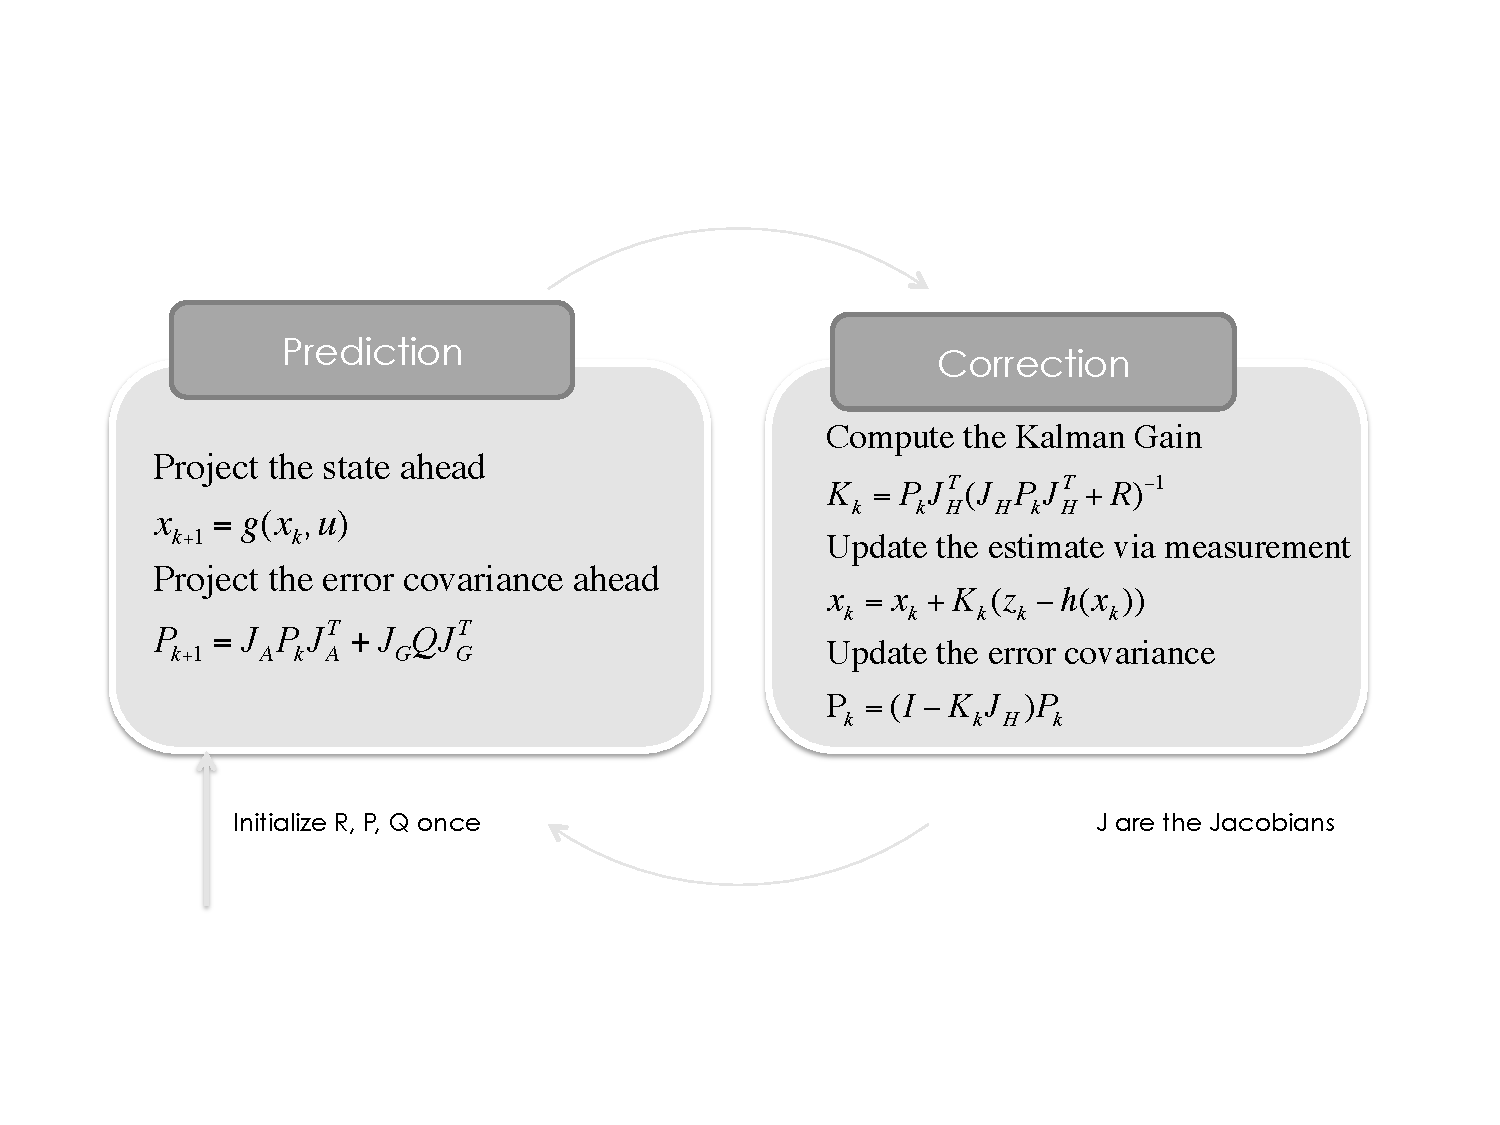
\includegraphics[width=3.4in]{images/Extended-Kalman-Filter-Step.pdf}
\caption{Extended Kalman Filter Step}
\label{EKF}
\end{figure}

Because the computational time is an important fact for real time state estimation, the EKF presented in this paper uses some calculations/conversions before the EKF itself, to reduce the complexity of the Jacobians, especially for the measurement function $h$.

\subsection{GNSS Position Accuracy}

In this paper, an adaptive extended Kalman Filter is introduced, which recalculates the measurement noise uncertainty for the position, based on the estimated position error ($EPE$), which is calculated by the GNSS receiver itself.

As \cite{Sharif} wrote, ``the EPE is a scalar indicating the precision of the receiver based on the deviation of the measurements from the mean of the measurement.''

For this reason, it cannot be used to determine a bias in the position measurement of the GNSS, but its relative error.

\begin{equation}EPE \sim \mathrm{HDOP} \cdot \mathrm{URA}(1 \sigma)\end{equation}

With $\text{HDOP}$ as the Horizontal Delution of Precision and $\text{URA}$ as the User Range Accuracy, which is a quantity that is transmitted in the navigation message and that is the predicted (not measured) statistical ranging accuracy.


\section{Extended Kalman Filter for CTRV dynamic with Attitude Estimation}

The implemented EKF estimates following state vector $x_k$, which is well known as the constant turn rate and velocity (CTRV) vehicle model + roll and pitch estimation:

\begin{equation}x_k= \left[ \begin{matrix}x \\ y \\ \psi \\ v \\ \dot \psi \\ \phi \\ \dot \phi \\ \Theta \\ \dot \Theta \end{matrix} \right] = \left[ \begin{matrix} \text{Position X (GNSS)} \\ \text{Position Y (GNSS)} \\ \text{Heading (GNSS)} \\ \text{Speed (GNSS)} \\ \text{Yaw Rate (IMU)} \\ \text{Pitch (IMU)} \\ \text{Pitchrate (IMU)} \\ \text{Roll (IMU)} \\ \text{Rollrate (IMU)} \end{matrix} \right]\end{equation}

As Schubert et. al. determined in \cite{Schubert2011}, "for ego motion estimation purposes which are characterized by a high update rate and the observability of $v$ and $\dot \psi$, model complexities beyond CTRV do not appear to be beneficial. However, the CTRV model shows its advantages as soon as a heading estimate is required."
The coordinate system is defined as shown in Fig.  \ref{KOS}.

\begin{figure}[ht]
\centering
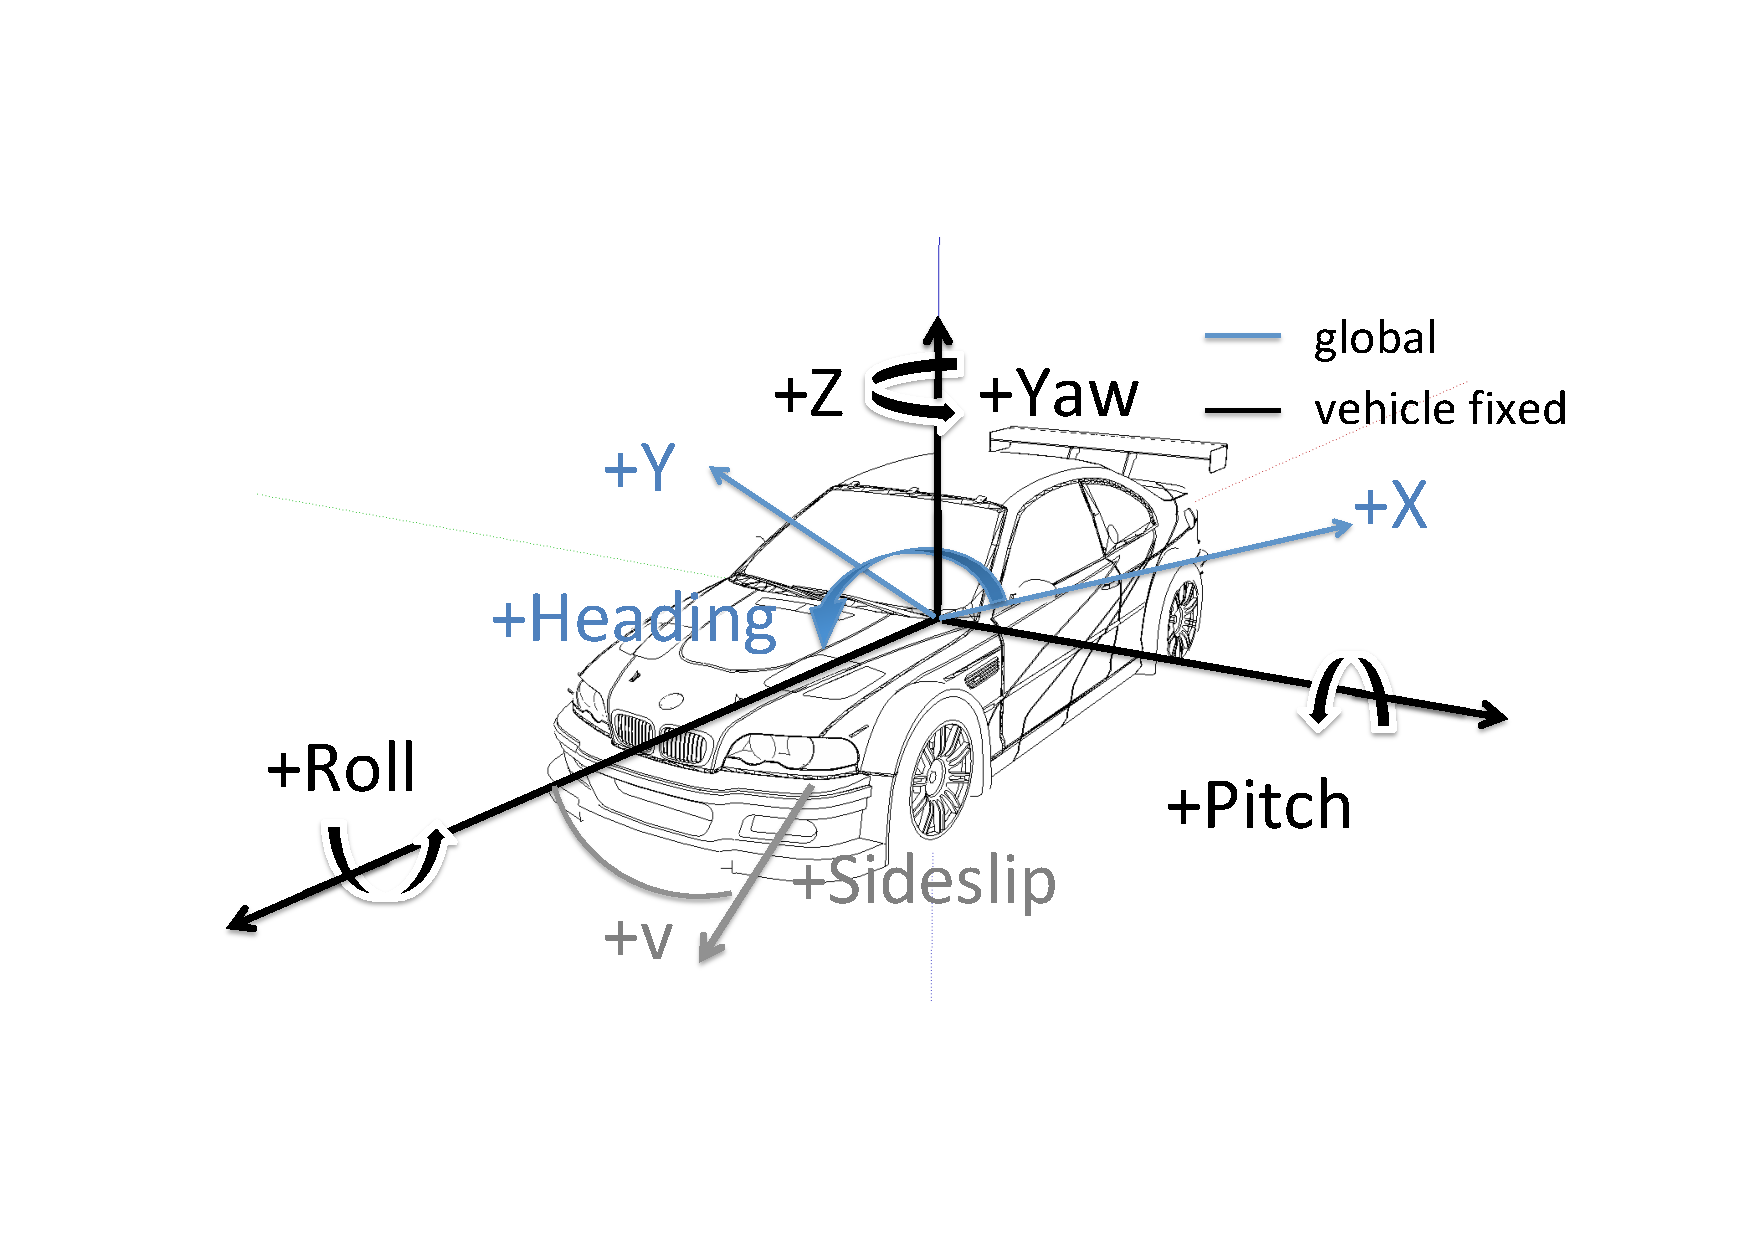
\includegraphics[width=2.6in]{images/Koordinatensystem-DIN70000.pdf}
\caption{Right hand coordinate system with z-axis to top}
\label{KOS}
\end{figure}

\subsection{Roll and Pitch Angle}

In \cite{Madgwick2010}, Madgwick presents an efficient orientation filter for inertial and inertial/magnetic sensor arrays. "The filter uses a quaternion representation, allowing accelerometer and magnetometer data to be used in an analytically derived and optimised gradient-descent algorithm to compute the direction of the gyroscope measurement error as a quaternion derivative.". The filter is implemented on the IMU and provides attitude information in quaternion representation in the global IMU coordinate system.

As mentioned there, the filter only estimates the correct attitude, if no external acceleration is actuating the vehicle. The calculated roll and pitch angles are actually just valid while standing still, not while accelerating/braking or cornering.

Madgwick recommended to adaptively choose convergence parameters, depending on absolute acceleration, influencing the IMU.

This paper lives this recommendation up and introduces an adaptively chosen weighting of roll and pitch angle and roll-/pitchrate, depending on the accelerations in x- or y-direction.

The roll and pitch angles, in vehicle coordinate system, are calculated with the quaternion ($Z_D=a-b\mathrm{i}_1-c\mathrm{i}_2-d\mathrm{i}_3$) output of the orientation filter \cite{Buchholz2013}.

\begin{equation}\label{rollangle}\phi = -\arcsin(2\cdot(a\cdot c - b \cdot d))\end{equation}
\begin{equation}\label{pitchangle}\theta = -\arctan\left(\frac{2\cdot(c\cdot d + a\cdot b)}{-(a^2-b^2-c^2+d^2)}\right)\end{equation}

\subsection{Position}

The position $x$ and $y$ is determined with a low cost GNSS receiver. The conversion between WGS84 $Lat$ and $Lon$ degrees to SI units is calculated as follows:
Assume the earth's radius with $R=\SI{6378}{\kilo\metre}$, then one degree of $Lon$ is
\begin{equation}arc = \cfrac{2 \pi\cdot R}{\SI{360}{\degree}} =  \SI{111.323}{\kilo\metre\per\degree}\end{equation}

One degree $Lat$ is \SI{111.32}{\kilo\metre} only near the equator. If moving to the poles, the value decreases until it is \SI{0}{\kilo\metre} on North- or Southpole. Taking the $\cos$ of the $Lat$ provides the correct length reduction (see Fig. \ref{LonLatEquatorNorthpole}).

\begin{figure}[ht]
\centering
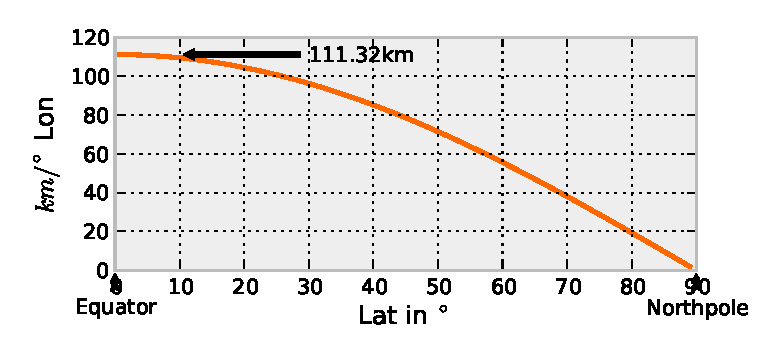
\includegraphics[width=2.5in]{images/Longitude-Cos-Latitude-Equator-Northpole}
\caption{Length of one degree of Longitude, depending on Latitude (WGS84)}
\label{LonLatEquatorNorthpole}
\end{figure}

\begin{equation}\label{deltax}\Delta x = arc\cdot\cos(Lat)\cdot\Delta Lon\end{equation}
\begin{equation}\label{deltay}\Delta y = arc\cdot\Delta Lat\end{equation}

With these equations the distance moved between two GNSS measurements can be calculated very accurate and additionally they simplify the state transition equations and the measurement function $h$, compared to other implementations, e.g. in \cite{Wender2008a}.

\subsection{State Control}

The rollrate $\dot \Theta$, the pitchrate $\dot \phi$, the yawrate $\dot \psi$ as well as the speed $v$ are state control variables.

\begin{equation}\label{controlinput}u_k=\left[\begin{matrix}v & \dot\psi & \dot\phi & \dot\Theta\end{matrix}\right]^T\end{equation}

The vector $u$ drives the state from one timestep $k$ to the next one.

\subsection{State Transition Function}

The state transition function $g(x_k, u_k)$ is defined with
\begin{equation}\label{statetransitionfunction}
x_{k+1}=\left[\begin{matrix}x + \frac{v}{\dot\psi} \left(- \sin{\left (\psi \right )} + \sin{\left (T \dot\psi + \psi \right )}\right)\\y + \frac{v}{\dot\psi} \left(\cos{\left (\psi \right )} - \cos{\left (T \dot\psi + \psi \right )}\right)\\T \dot\psi + \psi\\v\\\dot\psi\\T \dot\phi + \phi\\\dot\phi\\T \dot\Theta + \Theta\\\dot\Theta\end{matrix}\right]
\end{equation}
for $\dot \psi \neq 0$. For straight driving without curvature, the state transition function is
\begin{equation}
x_{k+1}=\left[\begin{matrix}x + v T \cdot \cos(\psi)\\y + v T \cdot \sin(\psi)\\ \psi \\v\\\ 0 \\T \dot\phi + \phi\\\dot\phi\\T \dot\Theta + \Theta\\\dot\Theta\end{matrix}\right]
\end{equation}

with $T$ as the time between two filtersteps. The Jacobians of the state transition with respect to the state and w.r.t. the control are listed in appendix.

\subsection{Process Noise Covariance Matrix Q}

As Kelly in \cite{Kelly1994} pointed out "a Kalman filter is a mathematical idealization that happens to be useful in practice. However, it is important to note that there is a big difference between an optimal estimate and an accurate estimate. In practical use, the uncertainty estimates take on the significance of relative weights of state estimates and measurements. So it is not so much important that uncertainty is absolutely correct as it is that it be relatively consistent across all models."

\begin{equation}Q=diag\label{Q}\left[\begin{matrix}\sigma_{v}^2 & \sigma_{{\dot\psi}}^2 & \sigma_{{\dot\phi}}^2 & \sigma_{{\dot\Theta}}^2 \end{matrix}\right]\end{equation}

Cross covariances resulting from deviation moments are assumed to be zero.

Assumptions for process noises for yawrate and velocity for a vehicle model are suggested in \cite{Kelly1994}. The process noise is best described with the question, how much the state can be propagated in one timestep by expected movement of the vehicle. So the maximal acceleration expected for a car might be $\SI{5}{\metre\per\square\second}$ under normal circumstances, so the $\sigma_v \approx a_\text{max}\cdot T$.
A typical maximal angular acceleration around vehicle z-axis might be $\SI{55}{\degree\per\square\second}$, which leads to a process noise of $\sigma_{\dot\psi} \approx \SI{55}{\degree\per\square\second} \cdot \frac{\pi}{180{,}0} \cdot T$.
The rotation around the pitch axis is much more dynamical, with typical angular accelerations of $\SI{200}{\degree\per\square\second}$. The rotation around the roll axis is in between and is assumed to be $\SI{130}{\degree\per\square\second}$.
The process noises for a $\SI{50}{\hertz}$ filter are listed in Table \ref{processnoisetable}.

\begin{table}[ht]
%% increase table row spacing, adjust to taste
\renewcommand{\arraystretch}{1.3}
% if using array.sty, it might be a good idea to tweak the value of
% \extrarowheight as needed to properly center the text within the cells
\caption{Process Noise Standard Deviations}
\label{processnoisetable}
\centering
%% Some packages, such as MDW tools, offer better commands for making tables
%% than the plain LaTeX2e tabular which is used here.
\begin{tabular}{c l c}
\hline
Parameter & Decribtion & Value\\
\hline
$\sigma_v$ & Velocity Process Noise & \SI{0.1}{\metre\per\second} \\
$\sigma_{\dot \psi}$ & Yawrate Process Noise & \SI{0.019}{\radian\per\second}\\
$\sigma_{\dot \phi}$ & Pitchrate Process Noise & \SI{0.07}{\radian\per\second}\\
$\sigma_{\dot \Theta}$ & Rollrate Process Noise & \SI{0.045}{\radian\per\second}\\
\hline
\end{tabular}
\end{table}

\subsection{Measurement Noise Covariance R}

Because the estimation of roll \eqref{rollangle} and pitch \eqref{pitchangle} is only valid for quasistatic situations (which is acutally not valid for a moving vehicle), the standard deviation for the calculated attitude angles $\sigma_r$ are adaptive to the accelerations $a_x$ and $a_y$.

The novel approach, presented in this paper, is the very easy to implement and fast to calculate weighting of the measurement noise covariance matrix $R$.

\begin{equation}\label{R}R=diag\left[\begin{matrix}\sigma_{x}^2 & \sigma_{y}^2 & \sigma_{\phi}^2 & \sigma_{\Theta}^2 \end{matrix}\right]\end{equation}

\subsubsection{Position Measurement Uncertainty}

In every EKF filterstep, the standard deviations for $\sigma_x$ and $\sigma_y$ are calculated, depending on the speed and additionally depending on the estimated position error ($EPE$), which is provided by the GNSS modul itself.
\begin{equation}\sigma_x^2 = \sigma_y^2 = \sigma_\text{v}^2 + \sigma_\text{EPE}^2\end{equation}
with
\begin{equation}\label{sigmav}\sigma_v = (v+\epsilon)^{-\xi}\end{equation}
\begin{equation}\label{sigmaepe}\sigma_\text{EPE} = \zeta \cdot EPE\end{equation}

The variables $\epsilon$, $\xi$ and $\zeta$ are tuneable parameters.

\subsubsection{Attitude Measurement Uncertainty}

The uncertainty for roll and pitch angle are adaptively calculated, depending on the vehicle accelerations in the appropriate directions.

\begin{equation}\label{sigmaroll}\sigma_\Theta=\left(\rho+\gamma\cdot a_y\right)^2\end{equation}

\begin{equation}\label{sigmapitch}\sigma_\psi=\left(\rho+\gamma\cdot a_x\right)^2\end{equation}

The variables $\rho$ and $\gamma$ are tuneable parameters.

\subsection{Measurement Function h}

Because of the simplifications \eqref{deltax} and \eqref{deltay}, the Jacobian of the measurement function $h$ with respect to the state $x_k$ is simple and computationally fast with 
\begin{equation}\label{hgps}J_H=\left[\begin{matrix}1 & 0 & 0 & 0 & 0 & 0 & 0 & 0 & 0\\0 & 1 & 0 & 0 & 0 & 0 & 0 & 0 & 0\\0 & 0 & 0 & 0 & 0 & 1 & 0 & 0 & 0\\0 & 0 & 0 & 0 & 0 & 0 & 0 & 1 & 0\end{matrix}\right]\end{equation}
when a new GNSS position measurement is available. In the practical implementation, the GNSS provide position information with \SI{10.0}{\hertz} and the EKF is estimating with \SI{50.0}{\hertz}. If no GNSS position information is available, the Jacobian of the measurement function $h$ with respect to the state $x_k$ is
\begin{equation}J_H=\left[\begin{matrix}0 & 0 & 0 & 0 & 0 & 0 & 0 & 0 & 0\\0 & 0 & 0 & 0 & 0 & 0 & 0 & 0 & 0\\0 & 0 & 0 & 0 & 0 & 1 & 0 & 0 & 0\\0 & 0 & 0 & 0 & 0 & 0 & 0 & 1 & 0\end{matrix}\right]\end{equation}

\section{Simulation}

\subsection{Simulation Setup}

To evaluate the adaptive EKF, a typical urban scenario, with shading from a buildings, as well as a vehicle stop, was simulated (see Fig. \ref{Testdata}).

\begin{figure}[ht]
\centering
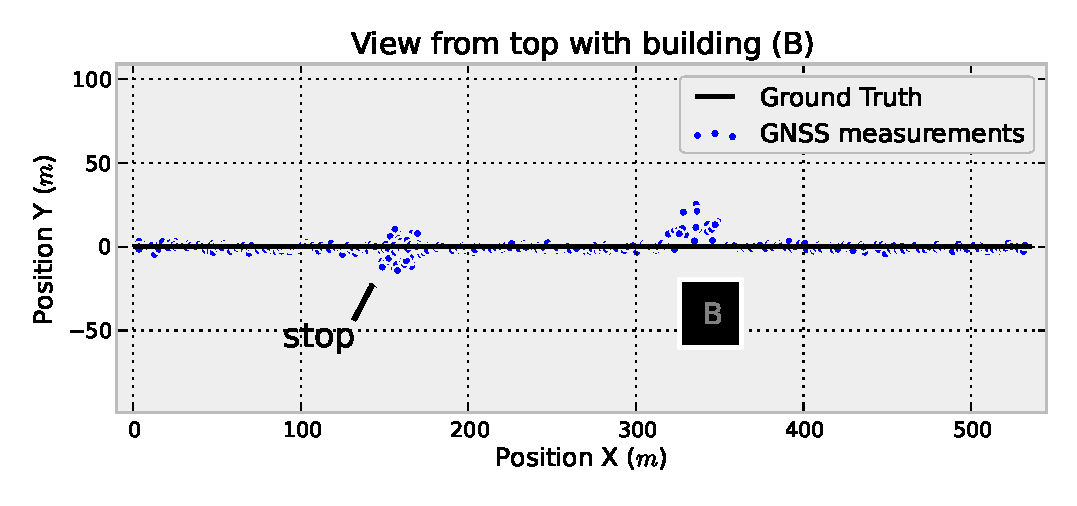
\includegraphics[width=3.2in]{images/Testdata}
\caption{Simulated GNSS measurements with vehicle stop and shading from a building (B) as well as ground truth}
\label{Testdata}
\end{figure}

The car starts at $x=0$, $y=0$ with $v=\SI{50.0}{\kilo\metre\per\hour}$ and decelerates until it stops. It is standing for $\SI{20}{\second}$ and accelerating until it reaches $v=\SI{50.0}{\kilo\metre\per\hour}$ again. Then it is passing a building, which disrupts the signal quality of the GNSS, so the position measurement is changed by $+\SI{15}{\metre}$ in $y$-direction, the $EPE$ is raised as well.

\begin{figure}[ht]
\centering
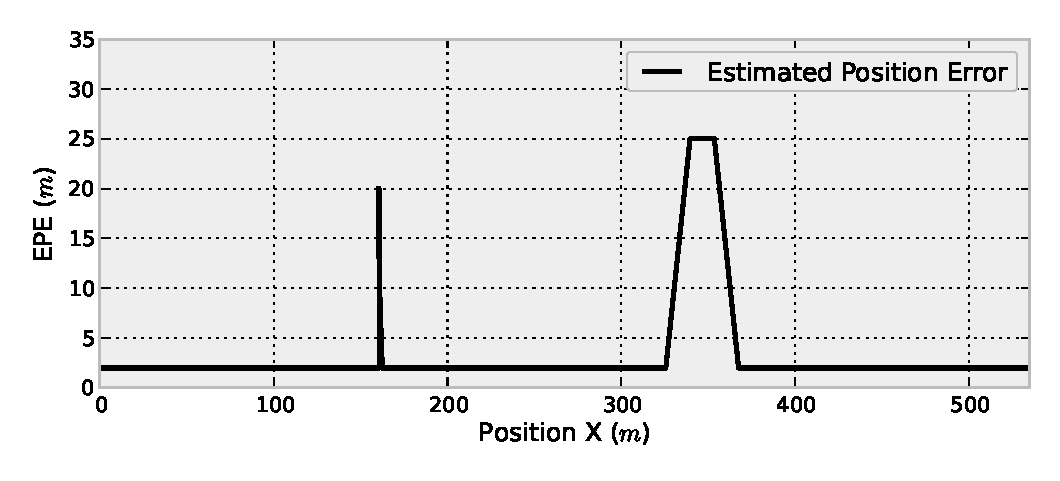
\includegraphics[width=3.2in]{images/Testdata-EPE}
\caption{Simulated GNSS Estimated Position Error}
\label{Testdata-EPE}
\end{figure}

\subsection{Parameter for Adaptive R}

The summand $\epsilon$ for \eqref{sigmav} is initialized with $\SI{1.0}{\metre\per\second}$, the exponent $\xi$ for \eqref{sigmav} with $500{,}0$ and the factor $\zeta$ for \eqref{sigmaepe} with $50{,}0$. The resulting values for $\sigma_x^2$ and $\sigma_y^2$ for a range of velocities and $EPE$s are shown in Fig. \ref{R1}.

\begin{figure}[ht]
\centering
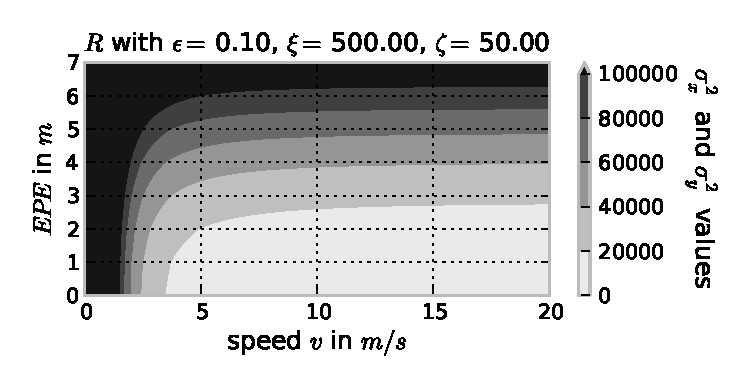
\includegraphics[width=3.0in]{images/R}
\caption{Values of $\sigma_x^2$ and $\sigma_y^2$ in $R$, depending on $v$ and $EPE$}
\label{R1}
\end{figure}

The factor $\rho$ for \eqref{sigmaroll} was initialized with $200{,}0$, the summand $\gamma$ was chosen to be $500{,}0$.

These parameters are empirically chosen and are subject to change for different cars or other driving scenarios or street quality.

\subsection{Simulation Results}

As one can see in Fig. \ref{CTRV-Position-Testdata}, the filter follows the trajectory of the GNSS measurements. If the EPE raises, the filter is more willing to trust the control input (see \eqref{controlinput}) instead of the position measurements.

\begin{figure}[ht]
\centering
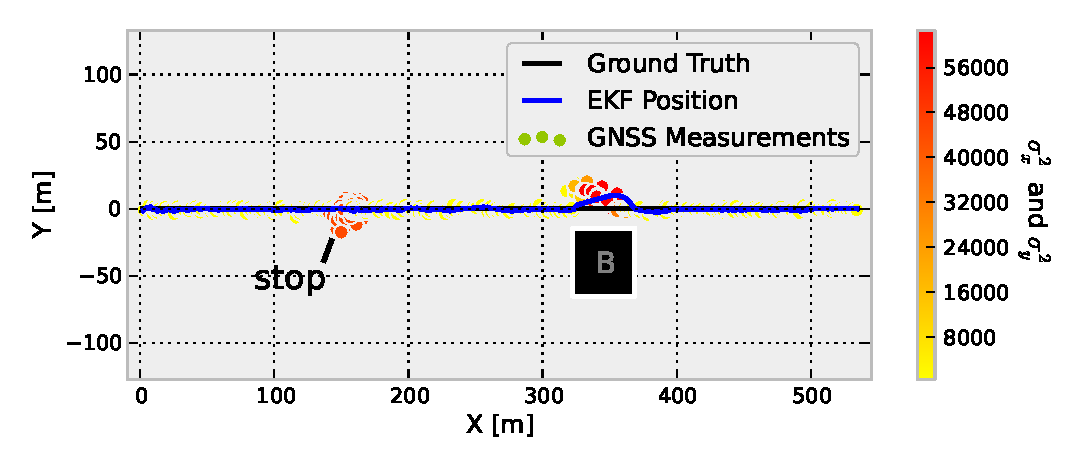
\includegraphics[width=3.5in]{images/Extended-Kalman-Filter-CTRV-Position-Testdata}
\caption{Measurements of GNSS with color coded value for $R$, depending on speed and EPE as well as estimated trajectory of the EKF}
\label{CTRV-Position-Testdata}
\end{figure}

To quantify the filter performance with respect to ground truth (GT) trajectory, the cross track error is introduced.

\begin{equation}\text{CTE}_x=x_{GT}-x\end{equation}
\begin{equation}\text{CTE}_y=y_{GT}-y\end{equation}

The sum of the square of the CTE for the simulation is a value to quantify the filter performance with respect to the correct trajectory estimation (see Fig. \ref{CTRV-CTE-Testdata}).

\begin{figure}[ht]
\centering
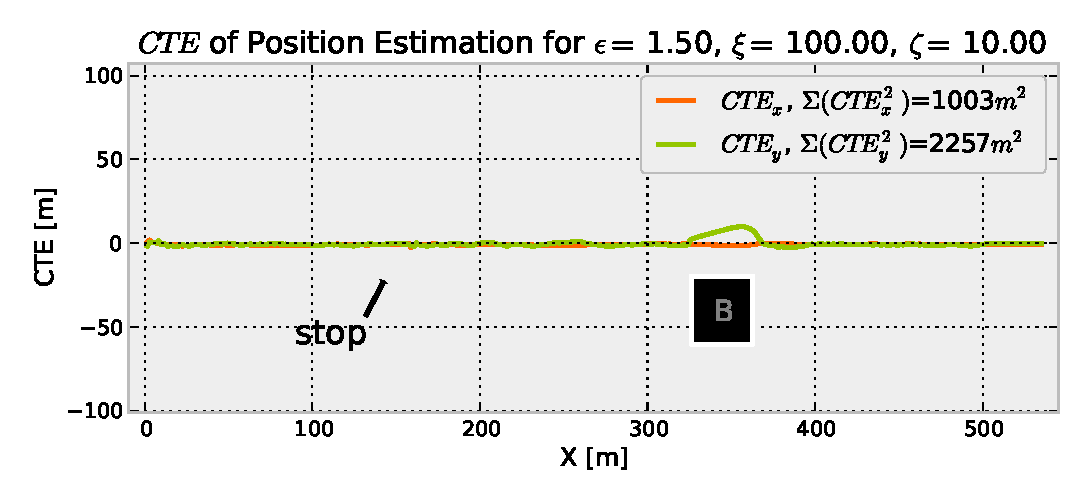
\includegraphics[width=3.5in]{images/Extended-Kalman-Filter-CTRV-CTE-Testdata}
\caption{Cross-Track-Error (not position estimate) with sum of the square}
\label{CTRV-CTE-Testdata}
\end{figure}

\subsection{Comparison to Standard EKF}

To compare the estimated trajectory with a non-adaptive EKF, the estimation was performed with several datasets for GNSS position measurements, generated by random Gaussian noise around the ground truth position.

The standard EKF was set up with static $\sigma_x^2=\SI{36}{\square\metre}$ and $\sigma_y^2=\SI{36}{\square\metre}$ values. The result is shown in Fig.  \ref{Boxplot}.

\begin{figure}[ht]
\centering
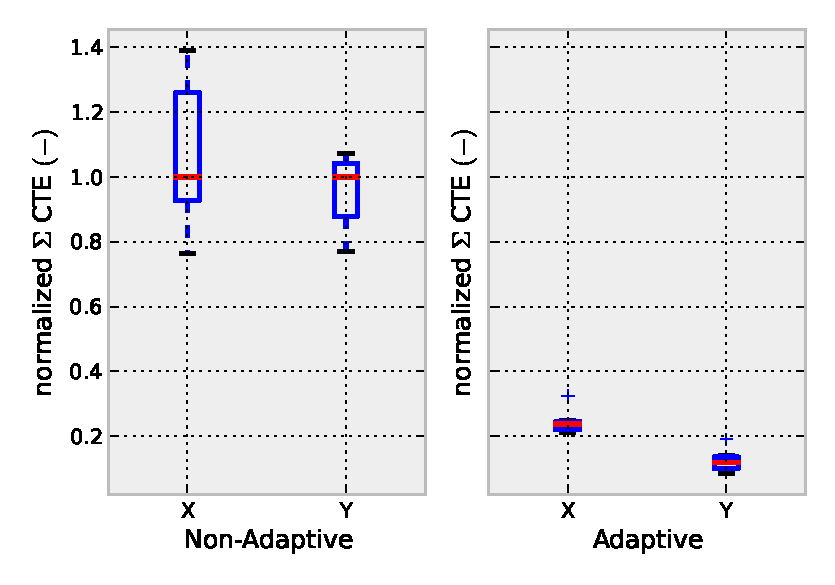
\includegraphics[width=3.0in]{images/CTE-Adaptive-NonAdaptive-Boxplot}
\caption{Comparison of the mean, upper and lower quantile of several runs for trajectory estimation and values for sum of squares of the CTE for the adaptive and the standard EKF}
\label{Boxplot}
\end{figure}

In comparison, the adaptive EKF reduces the $\Sigma \text{CTE}_x^2$ by $\SI{47}{\percent}$, the $\Sigma \text{CTE}_y^2$ by $\SI{59}{\percent}$, which for sure depends on the driving direction as well as on the chosen parameters.

Note, that the standard EKF could set up with high values for $R$ as well and may have better CTE values, but then, like for all filters, the dynamic is getting lost.

\section{Experimental Setup}

To test the performance of the filter with real GNSS data as well as a real car, the following sensores were used: LSM303   3-axis accelerometer and 3-axis magnetometer, ITG-3200 3-axis gyro, PA6H GNSS receiver. The sensors are available with the Tinkerforge IMU Brick\footnote{\url{http://www.tinkerforge.com/en/doc/Hardware/Bricks/IMU_Brick.html}} and GPS Bricklet\footnote{\url{http://www.tinkerforge.com/en/doc/Hardware/Bricklets/GPS.html}}.

For vehicle speed lower than $\SI{1,0}{\kilo\metre\per\hour}$ (GNSS), the speed and yawrate are set to zero, because the Doppler effect doesn't work for speed estimation in the GNSS receiver and turning while standing still is very unlikely.

\section{Experimental Results}

\begin{figure}[h!]
\centering
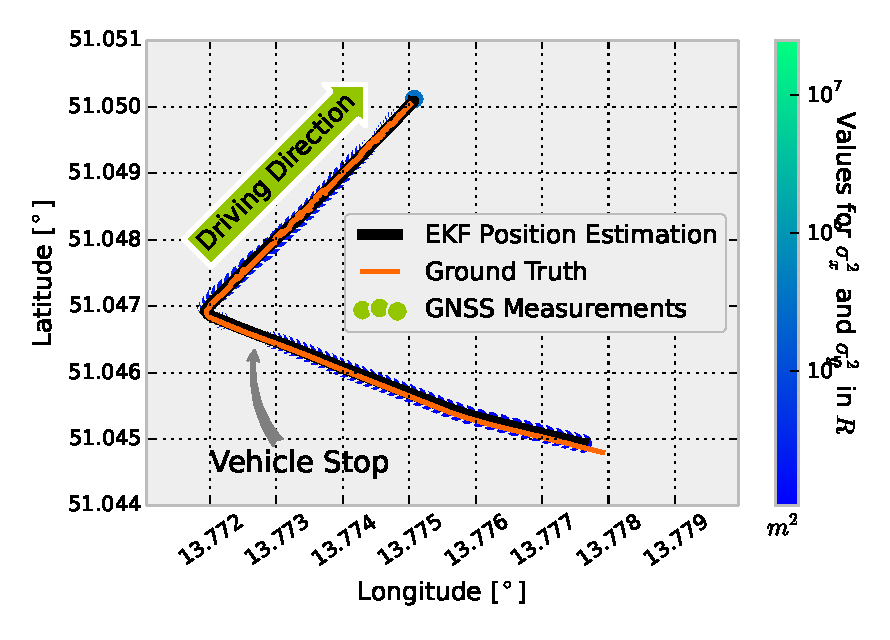
\includegraphics[width=3.4in]{images/Extended-Kalman-Filter-CTRV-Position}
\caption{Performed test drive with adaptive values of measurement uncertainty values for matrix $R$ (color)}
\label{ctrv-position}
\end{figure}

The state variables $x_k$ for the scenario were estimated as shown in Fig. \ref{ctrv-states}.

\begin{figure}[ht]
\centering
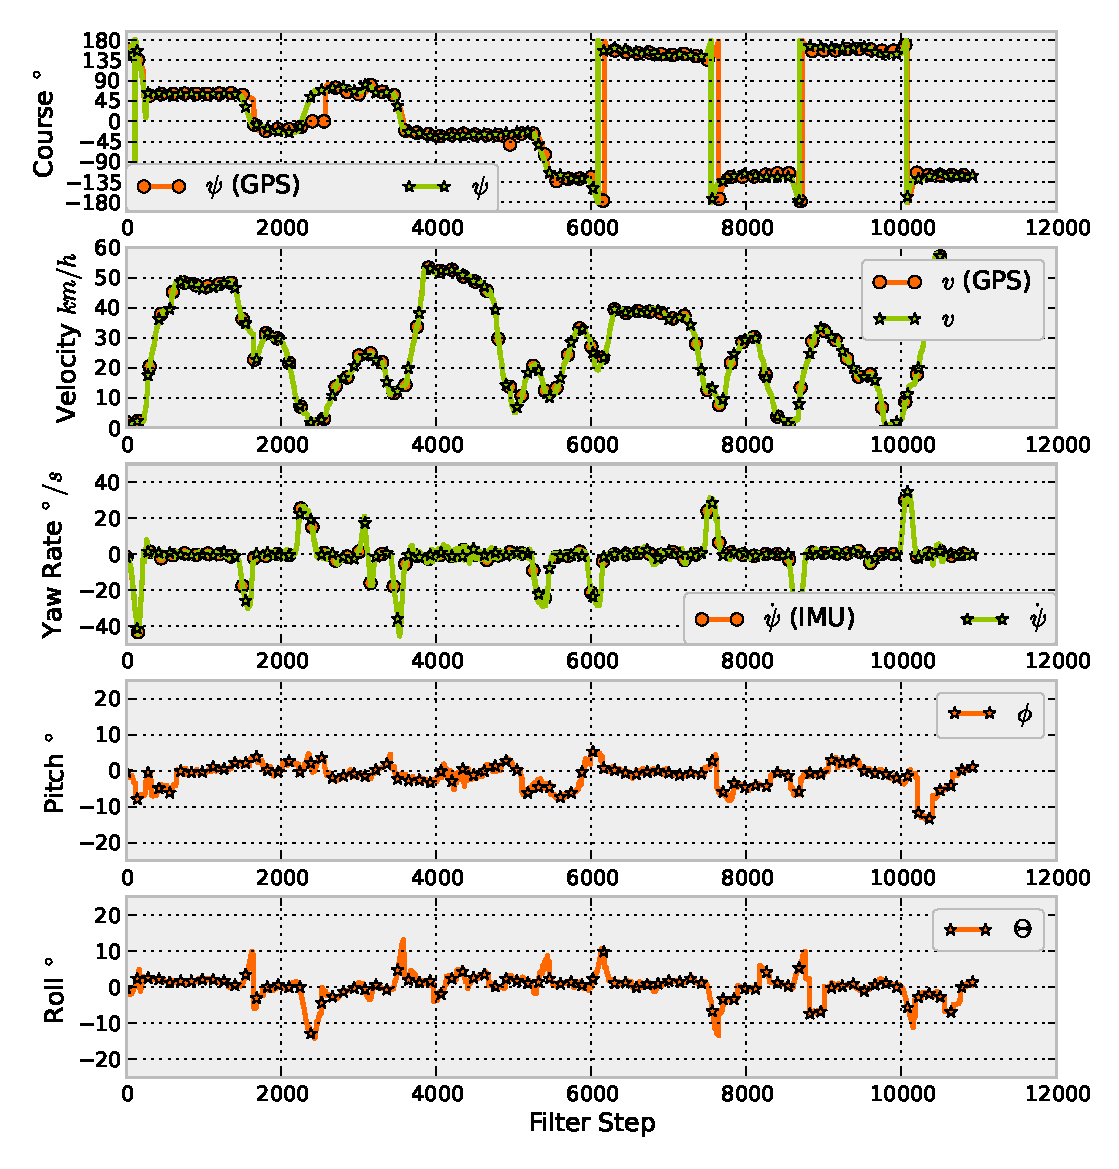
\includegraphics[width=3.5in]{images/Extended-Kalman-Filter-CTRV-Attitude-State-Estimates}
\caption{Estimated state variables $x_k$ for real world test drive}
\label{ctrv-states}
\end{figure}

As one can see, the stop before the last left turn got a high position measurement uncertainty, which in detail is shown in figure \ref{ctrv-position-detail}.

\begin{figure}[ht]
\centering
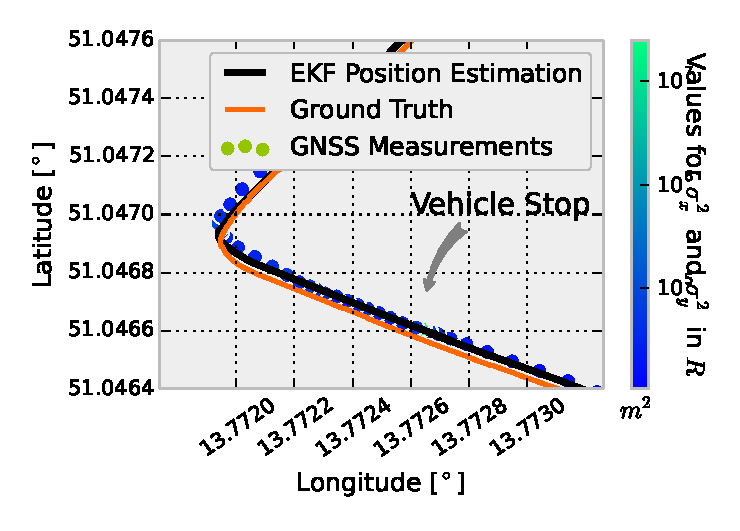
\includegraphics[width=3.2in]{images/Extended-Kalman-Filter-CTRV-Position-Detail}
\caption{Stop within the performed test drive with raised uncertainty for $R$ and position estimation from adaptive EKF}
\label{ctrv-position-detail}
\end{figure}


The state variables for vehicle speed and yawrate are nearly perfectly aligned, because they fit very well and they are state control variables as well. The state is forced to follow them.

While standing still, the heading measurement of the GNSS receiver is inaccurate (see Fig. \ref{ctrv-states} between filter step $k\approx2100\dotsc2300$). The filter performes very well on this situation and keeps the heading in the correct direction. The EKF position estimation (see Fig. \ref{ctrv-position-detail}) is not disturbed by inaccurate GNSS measurements while standing still and is dynamically responsive while driving. 

For the conducted test drive, the values for the measurement uncertainties in $R$ are calculated like shown in figure \ref{adaptive-R}.

\begin{figure}[ht]
\centering
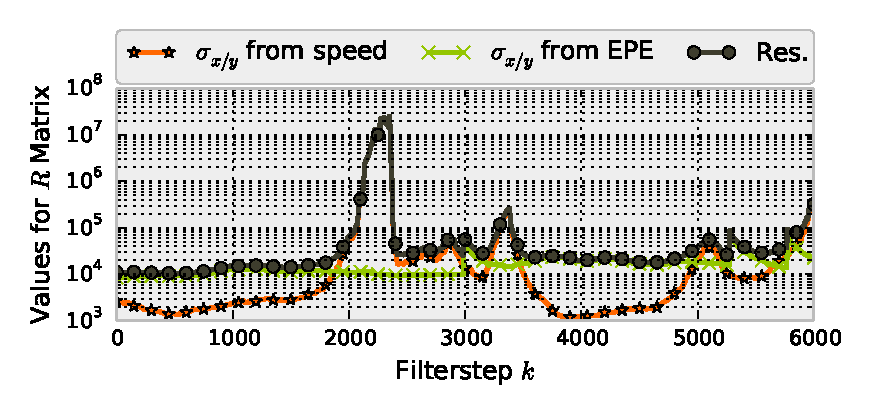
\includegraphics[width=3.2in]{images/Extended-Kalman-Filter-CTRV-Adaptive-R}
\caption{Values for adaptive $\sigma_v$, $\sigma_{EPE}$ and resulting $\sigma$ for $x$ and $y$}
\label{adaptive-R}
\end{figure}


% needed in second column of first page if using \IEEEpubid
%\IEEEpubidadjcol


% An example of a floating figure using the graphicx package.
% Note that \label must occur AFTER (or within) \caption.
% For figures, \caption should occur after the \includegraphics.
% Note that IEEEtran v1.7 and later has special internal code that
% is designed to preserve the operation of \label within \caption
% even when the captionsoff option is in effect. However, because
% of issues like this, it may be the safest practice to put all your
% \label just after \caption rather than within \caption{}.
%
% Reminder: the "draftcls" or "draftclsnofoot", not "draft", class
% option should be used if it is desired that the figures are to be
% displayed while in draft mode.
%
%\begin{figure}[!t]
%\centering
%\includegraphics[width=2.5in]{myfigure}
% where an .eps filename suffix will be assumed under latex, 
% and a .pdf suffix will be assumed for pdflatex; or what has been declared
% via \DeclareGraphicsExtensions.
%\caption{Simulation Results.}
%\label{fig_sim}
%\end{figure}

% Note that IEEE typically puts floats only at the top, even when this
% results in a large percentage of a column being occupied by floats.


% An example of a double column floating figure using two subfigures.
% (The subfig.sty package must be loaded for this to work.)
% The subfigure \label commands are set within each subfloat command,
% and the \label for the overall figure must come after \caption.
% \hfil is used as a separator to get equal spacing.
% Watch out that the combined width of all the subfigures on a 
% line do not exceed the text width or a line break will occur.
%
%\begin{figure*}[!t]
%\centering
%\subfloat[Case I]{\includegraphics[width=2.5in]{box}%
%\label{fig_first_case}}
%\hfil
%\subfloat[Case II]{\includegraphics[width=2.5in]{box}%
%\label{fig_second_case}}
%\caption{Simulation results.}
%\label{fig_sim}
%\end{figure*}
%
% Note that often IEEE papers with subfigures do not employ subfigure
% captions (using the optional argument to \subfloat[]), but instead will
% reference/describe all of them (a), (b), etc., within the main caption.


% An example of a floating table. Note that, for IEEE style tables, the 
% \caption command should come BEFORE the table. Table text will default to
% \footnotesize as IEEE normally uses this smaller font for tables.
% The \label must come after \caption as always.
%
%\begin{table}[!t]
%% increase table row spacing, adjust to taste
%\renewcommand{\arraystretch}{1.3}
% if using array.sty, it might be a good idea to tweak the value of
% \extrarowheight as needed to properly center the text within the cells
%\caption{An Example of a Table}
%\label{table_example}
%\centering
%% Some packages, such as MDW tools, offer better commands for making tables
%% than the plain LaTeX2e tabular which is used here.
%\begin{tabular}{|c||c|}
%\hline
%One & Two\\
%\hline
%Three & Four\\
%\hline
%\end{tabular}
%\end{table}


% Note that IEEE does not put floats in the very first column - or typically
% anywhere on the first page for that matter. Also, in-text middle ("here")
% positioning is not used. Most IEEE journals use top floats exclusively.
% Note that, LaTeX2e, unlike IEEE journals, places footnotes above bottom
% floats. This can be corrected via the \fnbelowfloat command of the
% stfloats package.



\section{Conclusion}
In this paper we presented a novel approach to adaptively calculate the measurement uncertainty for an improved position and attitude estimation, based on the Estimated Position Error and the speed, determined by the low cost GNSS receiver.
We explained the basics and used some empirically chosen values to parametrize the filter. With that, we showed with simulated data, that the filter performes significantly better than a standard Extended Kalman Filter. Based on that, we conducted test drives and used the developed Adaptive EKF for a real world dataset, which proved its ability to improve the position estimation with partly bad signal quality. In addition to that, the filter also performs pretty well on dynamic situations and is not loosing the ability to follow dynamic vehicle movements.
The filter cannot be used to get rid of bias in position estimation, because the EPE from GNSS has, by definition, no information about static drift of the position information.
The presented filter can be used to get significantly better results while standing still or driving slowly as well as keeping the heading fixed while do so.
Additionally, the attitude of the vehicle is estimated, based on the filter presented in \cite{Madgwick2010} in rest position and with angular velocity sensors from IMU while driving.

% if have a single appendix:
%\appendix[Proof of the Zonklar Equations]
% or
%\appendix  % for no appendix heading
% do not use \section anymore after \appendix, only \section*
% is possibly needed

% use appendices with more than one appendix
% then use \section to start each appendix
% you must declare a \section before using any
% \subsection or using \label (\appendices by itself
% starts a section numbered zero.)
%

% use section* for acknowledgement
\section*{Acknowledgment}

%The authors would like to thank the Free State of Saxony and the European Union, which funded the research from the ESF fond.
T.b.d.

\appendices
\section{Programm Code and EKF Implementation}
The implemenented EKF code as well as all figures and the data used in this paper can be found online at t.b.d %\url{http://balzer82.github.com/MMAR14}

\section{Jacobians}

The Jacobian of the state transition \eqref{statetransitionfunction} function with respect to the state $x_k$ is defined with

\begin{equation}
J_A=\left[\begin{matrix}1 & 0 & J_{A,13} & J_{A,14} & J_{A,15} & 0 & 0 & 0 & 0\\0 & 1 & J_{A,23} & J_{A,24} & J_{A,25} & 0 & 0 & 0 & 0\\0 & 0 & 1 & 0 & T & 0 & 0 & 0 & 0\\0 & 0 & 0 & 1 & 0 & 0 & 0 & 0 & 0\\0 & 0 & 0 & 0 & 1 & 0 & 0 & 0 & 0\\0 & 0 & 0 & 0 & 0 & 1 & T & 0 & 0\\0 & 0 & 0 & 0 & 0 & 0 & 1 & 0 & 0\\0 & 0 & 0 & 0 & 0 & 0 & 0 & 1 & T\\0 & 0 & 0 & 0 & 0 & 0 & 0 & 0 & 1\end{matrix}\right]
\end{equation}

with

\begin{equation}J_{A,13}=\frac{v}{\dot\psi} \left(- \cos{\left (\psi \right )} + \cos{\left (T \dot\psi + \psi \right )}\right)\end{equation}
\begin{equation}J_{A,14}=\frac{1}{\dot\psi} \left(- \sin{\left (\psi \right )} + \sin{\left (T \dot\psi + \psi \right )}\right)\end{equation}
\begin{equation}J_{A,15}=\frac{T v}{\dot\psi} \cos{\left (T \dot\psi + \psi \right )} - \frac{v}{\dot\psi} \cdot J_{A,14}\end{equation}
\begin{equation}J_{A,23}=\frac{v}{\dot\psi} \left(- \sin{\left (\psi \right )} + \sin{\left (T \dot\psi + \psi \right )}\right)\end{equation}
\begin{equation}J_{A,24}=\frac{1}{\dot\psi} \left(\cos{\left (\psi \right )} - \cos{\left (T \dot\psi + \psi \right )}\right)\end{equation}
\begin{equation}J_{A,25}=\frac{T v}{\dot\psi} \sin{\left (T \dot\psi + \psi \right )} - \frac{v}{\dot\psi}\cdot J_{A,24}\end{equation}

The Jacobian of the state transition function with respect to the control is

\begin{equation}J_G=\left[\begin{matrix}J_{G,11} & J_{G,12} & 0 & 0\\ J_{G,21} & J_{G,22} & 0 & 0\\0 & T & 0 & 0\\1 & 0 & 0 & 0\\0 & 1 & 0 & 0\\0 & 0 & T & 0\\0 & 0 & 1 & 0\\0 & 0 & 0 & T\\0 & 0 & 0 & 1\end{matrix}\right]\end{equation}
with
\begin{equation}J_{G,11}=\frac{1}{\dot\psi} \left(- \sin{\left (\psi \right )} + \sin{\left (T \dot\psi + \psi \right )}\right)\end{equation}
\begin{equation}J_{G,12}=\frac{T v}{\dot\psi} \cos{\left (T \dot\psi + \psi \right )} - \frac{v}{\dot\psi} \cdot J_{G,11}\end{equation}
\begin{equation}J_{G,21}=\frac{1}{\dot\psi} \left(\cos{\left (\psi \right )} - \cos{\left (T \dot\psi + \psi \right )}\right)\end{equation}
\begin{equation}J_{G,22}=\frac{T v}{\dot\psi} \sin{\left (T \dot\psi + \psi \right )} - \frac{v}{\dot\psi} \cdot J_{G,21}\end{equation}


% you can choose not to have a title for an appendix
% if you want by leaving the argument blank

% Can use something like this to put references on a page
% by themselves when using endfloat and the captionsoff option.
\ifCLASSOPTIONcaptionsoff
  \newpage
\fi



% trigger a \newpage just before the given reference
% number - used to balance the columns on the last page
% adjust value as needed - may need to be readjusted if
% the document is modified later
%\IEEEtriggeratref{8}
% The "triggered" command can be changed if desired:
%\IEEEtriggercmd{\enlargethispage{-5in}}

% references section

% can use a bibliography generated by BibTeX as a .bbl file
% BibTeX documentation can be easily obtained at:
% http://www.ctan.org/tex-archive/biblio/bibtex/contrib/doc/
% The IEEEtran BibTeX style support page is at:
% http://www.michaelshell.org/tex/ieeetran/bibtex/
\bibliography{bibtex/bib/IEEEabrv.bib,bibtex/bib/library.bib}{}
\bibliographystyle{IEEEtran}
% argument is your BibTeX string definitions and bibliography database(s)
%\bibliography{}
%
% <OR> manually copy in the resultant .bbl file
% set second argument of \begin to the number of references
% (used to reserve space for the reference number labels box)
%\begin{thebibliography}{1}

%\bibitem{IEEEhowto:kopka}
%H.~Kopka and P.~W. Daly, \emph{A Guide to \LaTeX}, 3rd~ed.\hskip 1em plus
%  0.5em minus 0.4em\relax Harlow, England: Addison-Wesley, 1999.
%
%\end{thebibliography}

% biography section
% 
% If you have an EPS/PDF photo (graphicx package needed) extra braces are
% needed around the contents of the optional argument to biography to prevent
% the LaTeX parser from getting confused when it sees the complicated
% \includegraphics command within an optional argument. (You could create
% your own custom macro containing the \includegraphics command to make things
% simpler here.)

%\begin{IEEEbiography}[{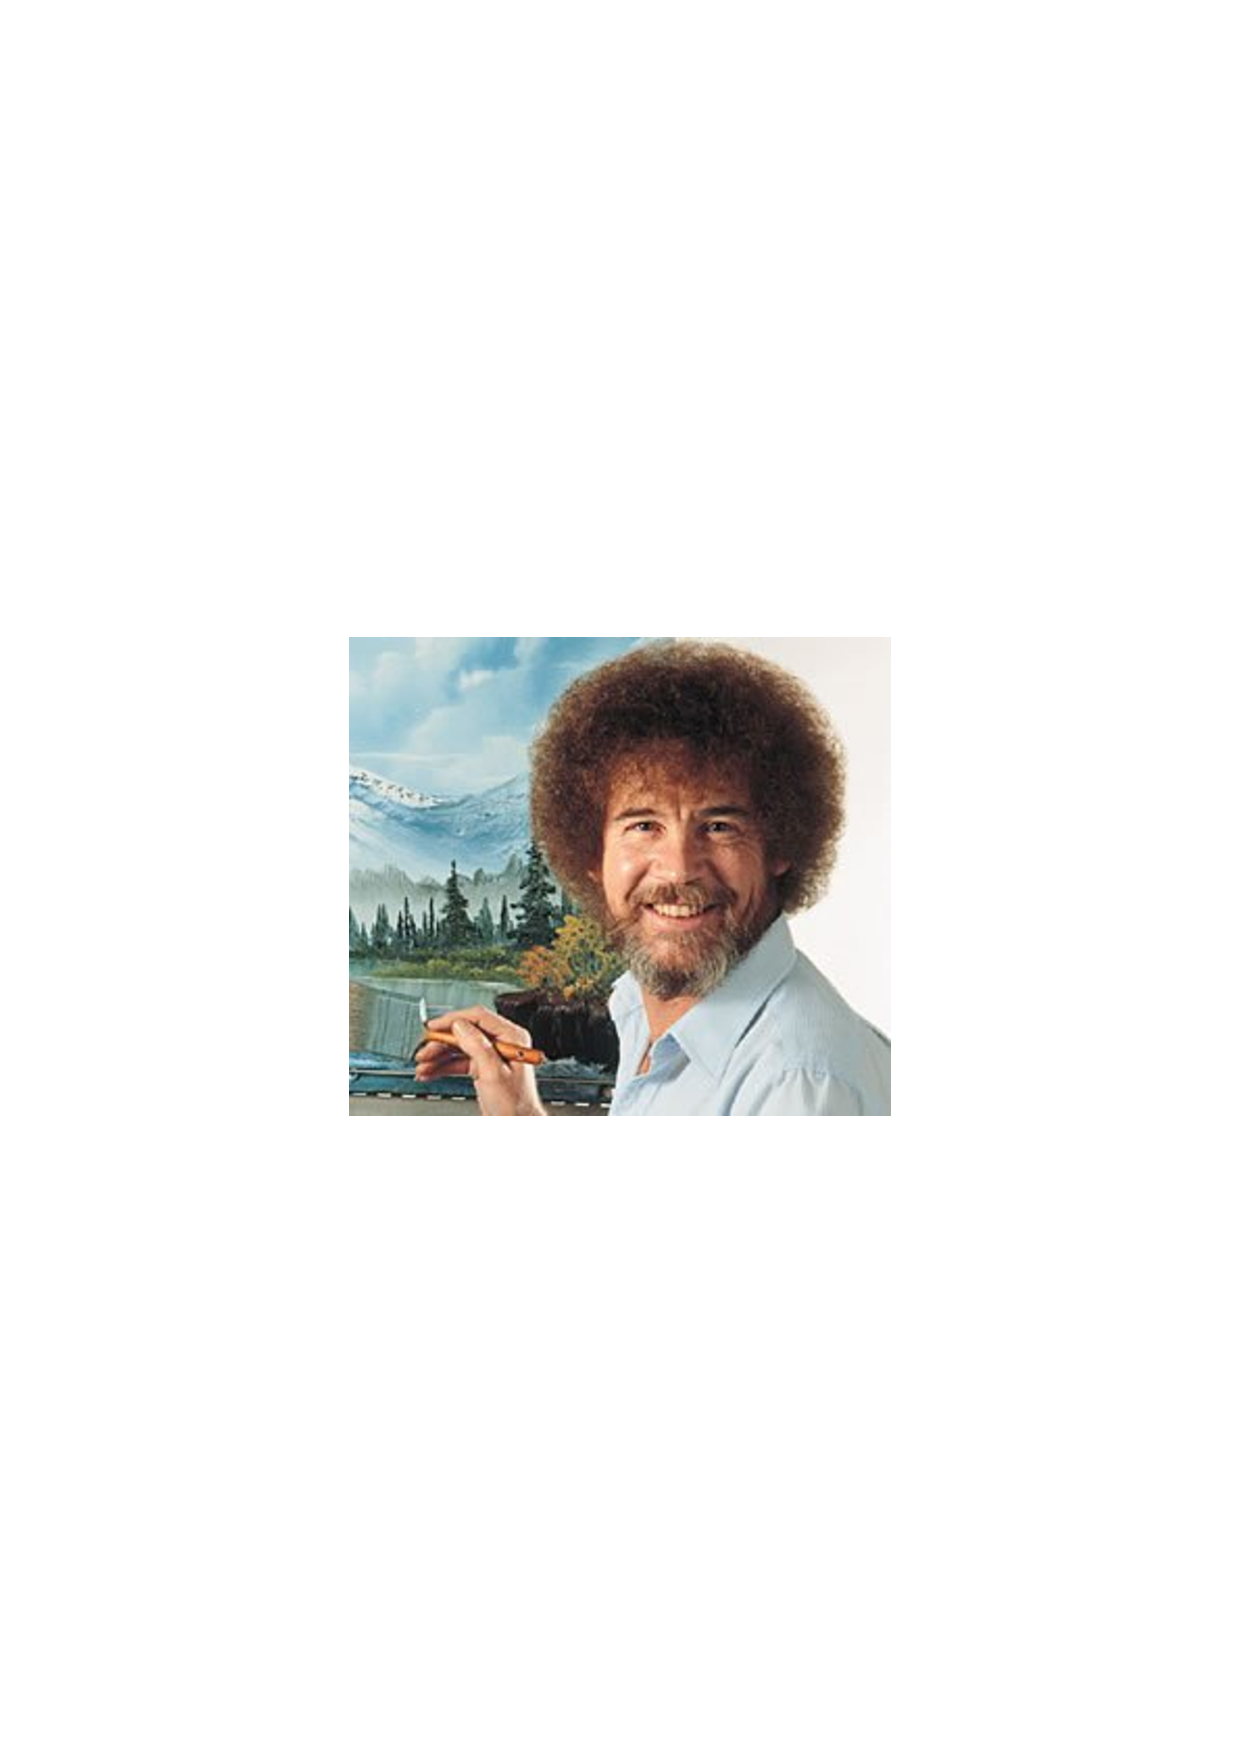
\includegraphics[width=1in,height=1.25in,clip,keepaspectratio]{fotos/Profilbild_Bob_Ross.pdf}}]{Paul~Balzer}Ph.D. Student at the University of Applied Sciences Dresden in cooperation with the Technical University Dresden
%\end{IEEEbiography}

%\begin{IEEEbiography}{Toralf~Trautmann}, Dr. rer. nat., Professor for vehicle mechatronics at the University of Applied Sciences Dresden
%\end{IEEEbiography}

%\begin{IEEEbiography}{Oliver~Michler}, Prof. Dr.-Ing., Chair of Transport Systems Information Technology, which is part of  Institute for Traffic Telematics at the Faculty of Transportation and Traffic Sciences ``Friedrich List'' of the Technical University Dresden
%\end{IEEEbiography}

% or if you just want to reserve a space for a photo:

%\begin{IEEEbiography}{Paul Balzer}
%Ph.D. student at the HTW Dresden in cooperation with the TU Dresden
%\end{IEEEbiography}



% insert where needed to balance the two columns on the last page with
% biographies
%\newpage

% You can push biographies down or up by placing
% a \vfill before or after them. The appropriate
% use of \vfill depends on what kind of text is
% on the last page and whether or not the columns
% are being equalized.

%\vfill

% Can be used to pull up biographies so that the bottom of the last one
% is flush with the other column.
%\enlargethispage{-5in}



% that's all folks
\end{document}